\section{Problem 3}
\textit{A correlation coefficient of 0.7 is usually taken as sufficient for uncorrelated signals – explain why using the figure 2.42. b) are there much to conclude from the in-depth investigation shown in figure 2.59 to 2.63?}\\

\begin{figure}[!h]
  \centering
  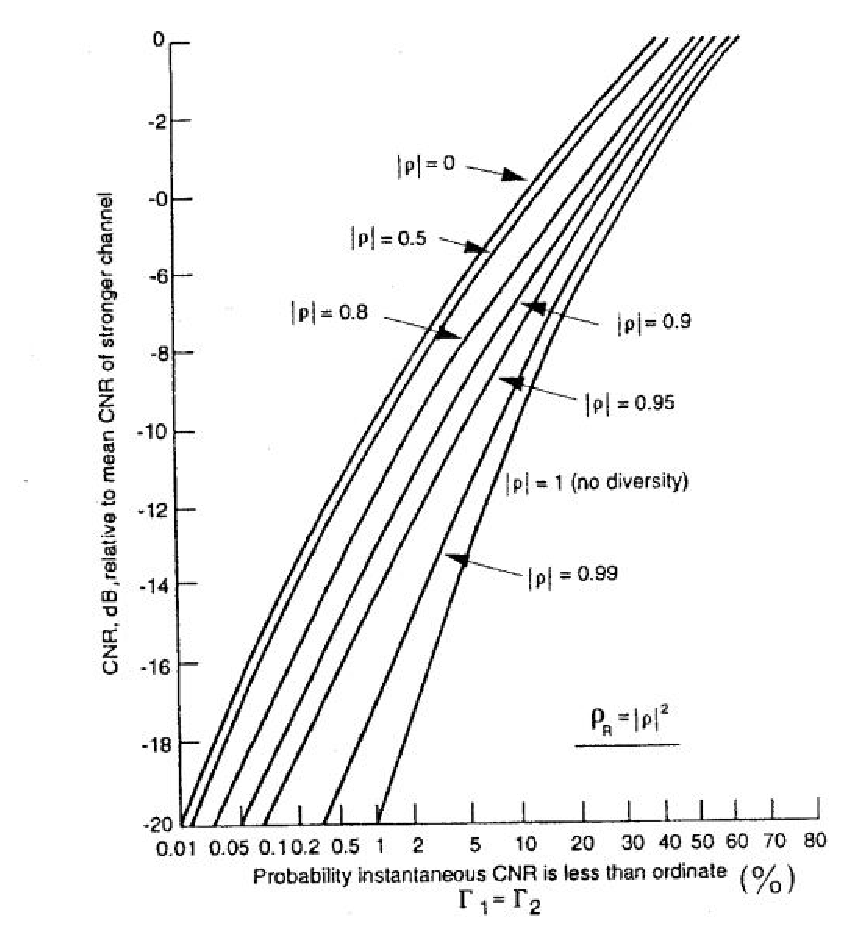
\includegraphics[width=10cm]{selective_combining.eps}
  \caption{Figure showing the influence of the correlation coefficient for selective combining of two signals (from Mobile Antenna System Handbook, K. Fujimo, J.R. James, p.80).}
  \label{fig:selective_combining}
\end{figure}

\begin{figure}[!h]
  \centering
  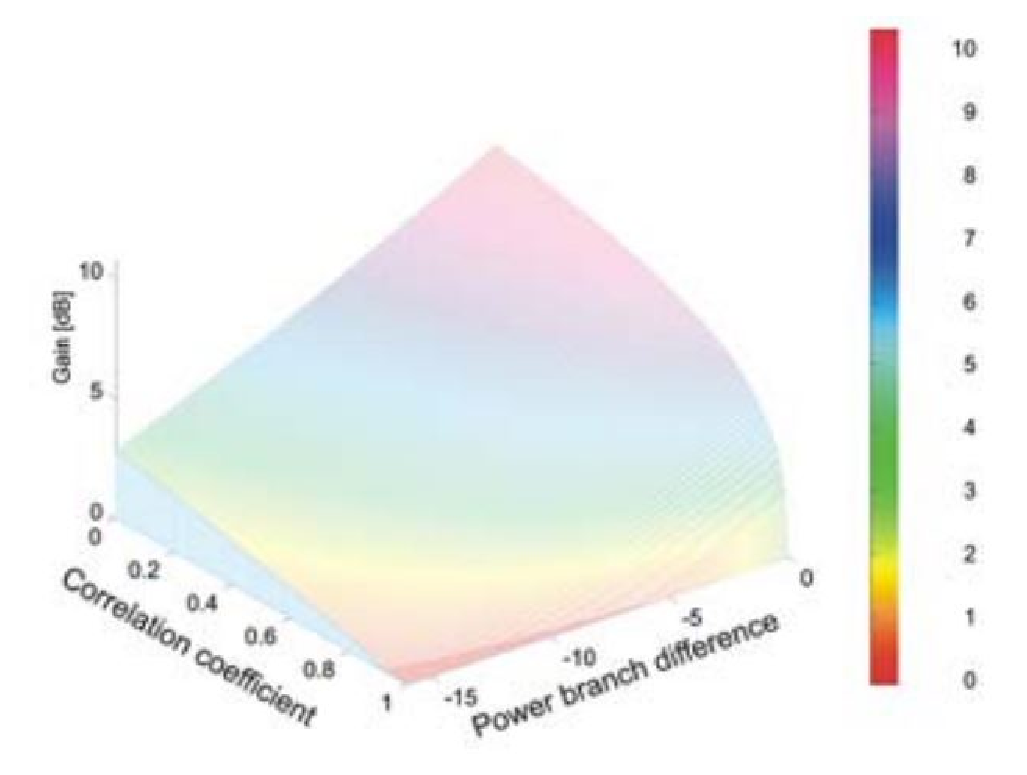
\includegraphics[width=10cm]{selective_combining2.eps}
  \caption{Diversity gain for selective combining (from the script).}
  \label{fig:selective_combining2}
\end{figure}

As can be seen from \figref{fig:selective_combining} the probability, that the CNR is lower than a given CNR bound is not changing rapidly when moving from the $\rho=0$ (fully uncorrelated) to the $\rho=0.7$ graph. For example one could compare the values for \SI{-10}{\decibel}: From $\rho=0.7$ to $\rho=0$ we only gain \SI{1}{\percent} (from \SI{2}{\percent} to \SI{1}{\percent}), while we lose a lot when going from $\rho=0.7$ to the fully correlated, non-diversity case ($\rho=1$), where we arrive at \SI{10}{\percent}. The same can be seen in \figref{fig:selective_combining2}, where it is easily notable when comparing the values for a \SI{0}{\decibel} power branch difference (MEG). Again, from $\rho=0.7$ to $\rho=0$, the diversity gain does not change to much, but we can register a significant loss from $\rho=0.7$ to $\rho=1$. Thus it can be concluded, that a correlation coefficient of 0.7 is sufficient. \\


\textit{b) are there much to conclude from the in-depth investigation shown in figure 2.59 to 2.63?}\\

No, since the in-depth investigation focusses too much on very small scaled effects, which do not play any bigger role compared to the effects discussed in the previous tasks.